\section{Experiment 3 : DNS}
% Experiment 3-1
\subsection{DNS : Traing DNS with Wireshark \#1}
    \subsubsection*{Experiment Results}
         \vspace{-4mm}
    	\begin{figure}[!h]\centering
    % 		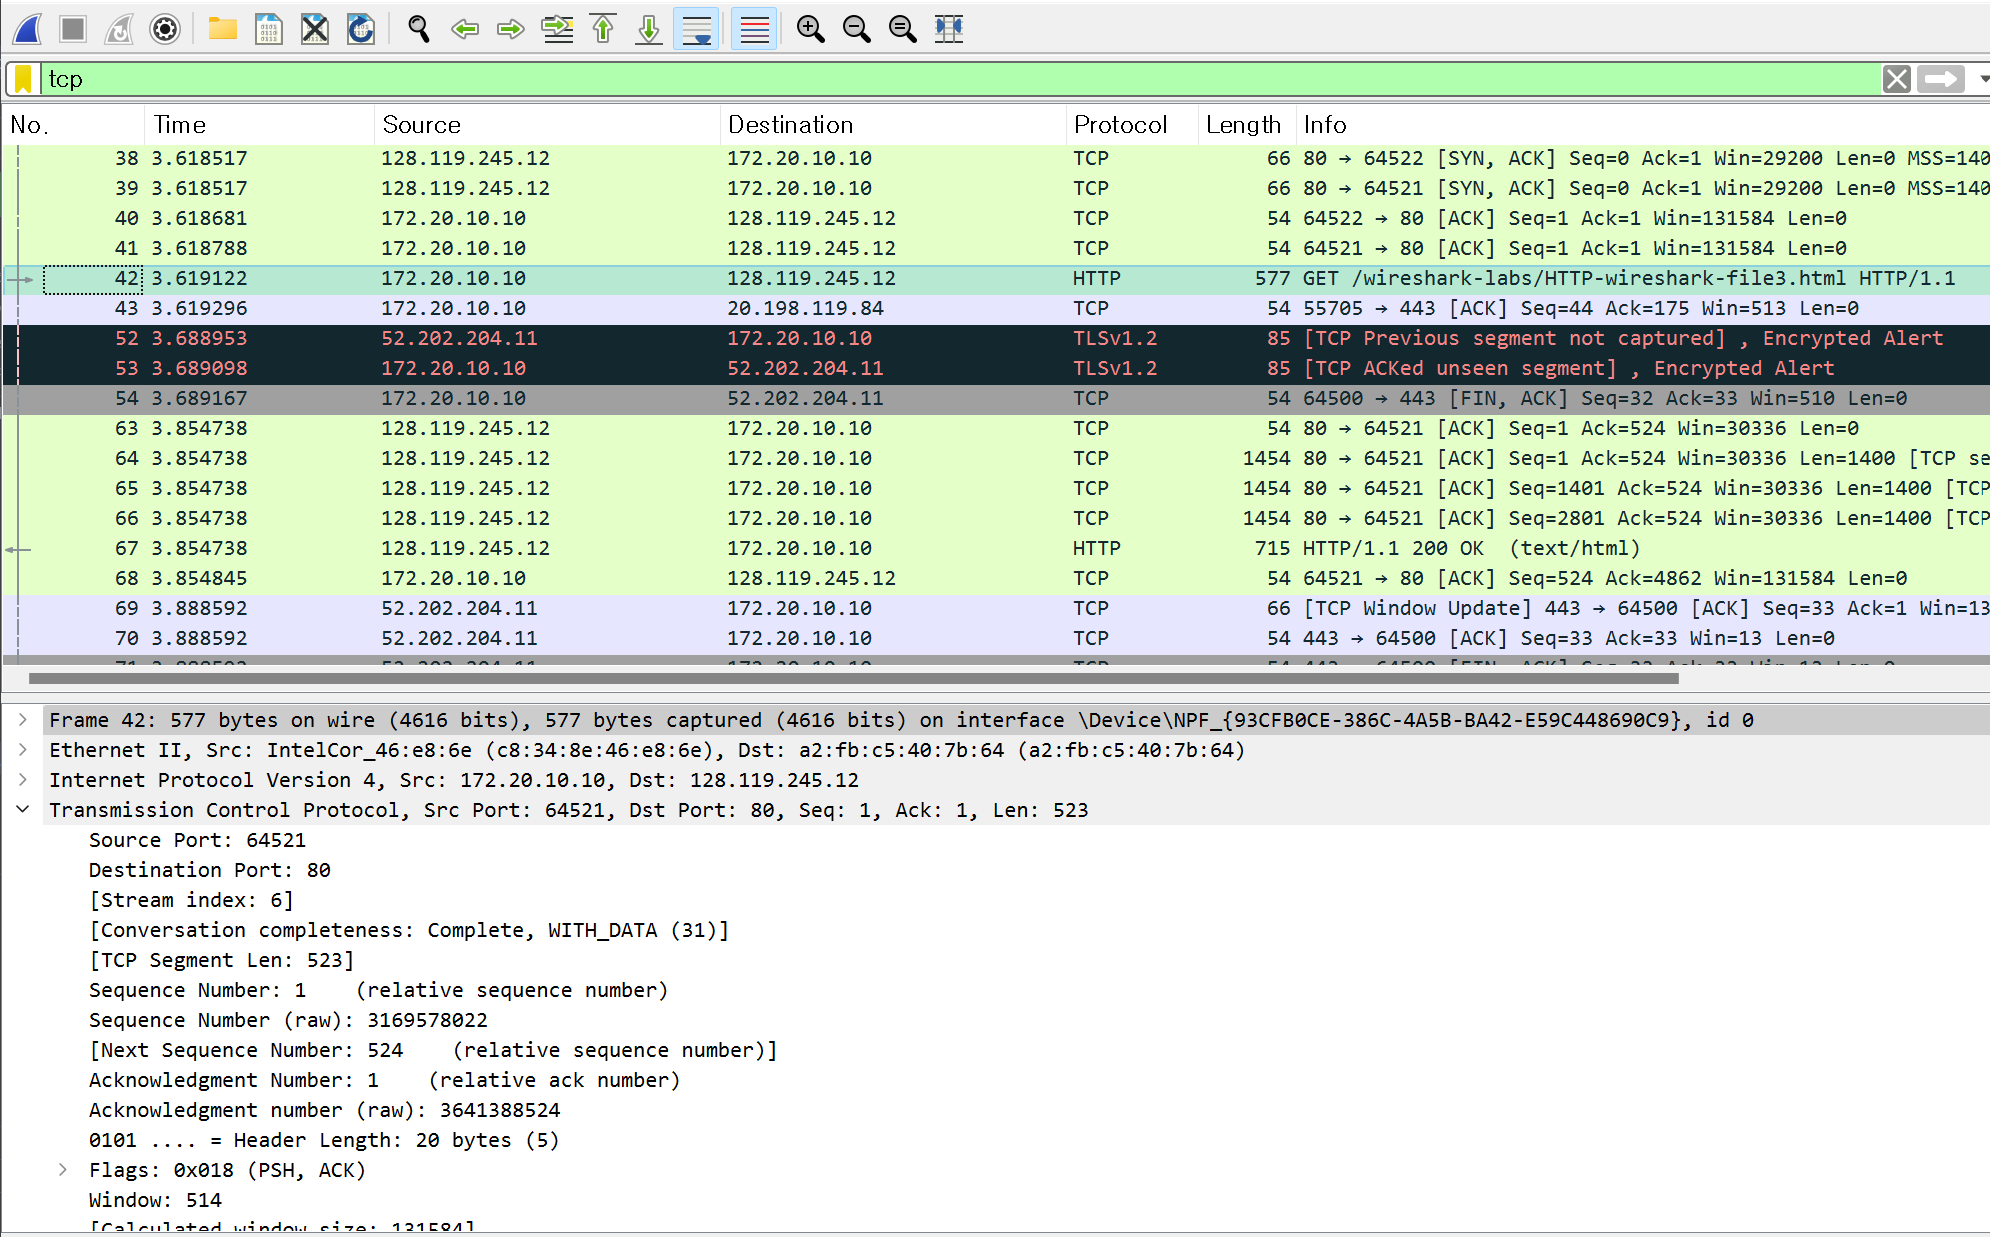
\includegraphics[width=.95\textwidth]{image/week01/2-9.png}
    		\caption{Wireshark Screenshot}
    	\end{figure}
        \vspace{-4mm}  
    \subsubsection*{Questions}
        \begin{enumerate}[label=\bfseries Problem \arabic*:,leftmargin=*,labelindent=1em]
        % \addtocounter{enumi}{11}
            \item Locate the DNS query and response messages. Are then sent over UDP or TCP?\\[0.2mm]
            \soln
            
            \item What is the destination port for the DNS query message? 
            What is the source port of DNS response message?\\[0.2mm]
            \soln
            
            \item To what IP address is the DNS query message sent? 
            Use ipconfig to determine the IP address of your local DNS server. 
            Are these two IP addresses the same?\\[0.2mm]
            \soln
            
            \item Examine the DNS query message. What “Type” of DNS query is it? 
            Does the query message contain any “answers”?\\[0.2mm]
            \soln
            
            \item Examine the DNS response message. How many “answers” are provided? 
            What do each of these answers contain?\\[0.2mm]
            \soln
            
            \item Consider the subsequent TCP SYN packet sent by your host.
            Does the destination IP address of the SYN packet correspond to any of the IP addresses 
            provided in the DNS response message?\\[0.2mm]
            \soln
            
            \item This web page contains images. Before retrieving each image, 
            does your host issue new DNS queries?\\[0.2mm]
            \soln
            
        \end{enumerate}
% Experiment 3-2
\subsection{DNS : Traing DNS with Wireshark \#2}
    \subsubsection*{Experiment Results}
         \vspace{-4mm}
    	\begin{figure}[!h]\centering
    % 		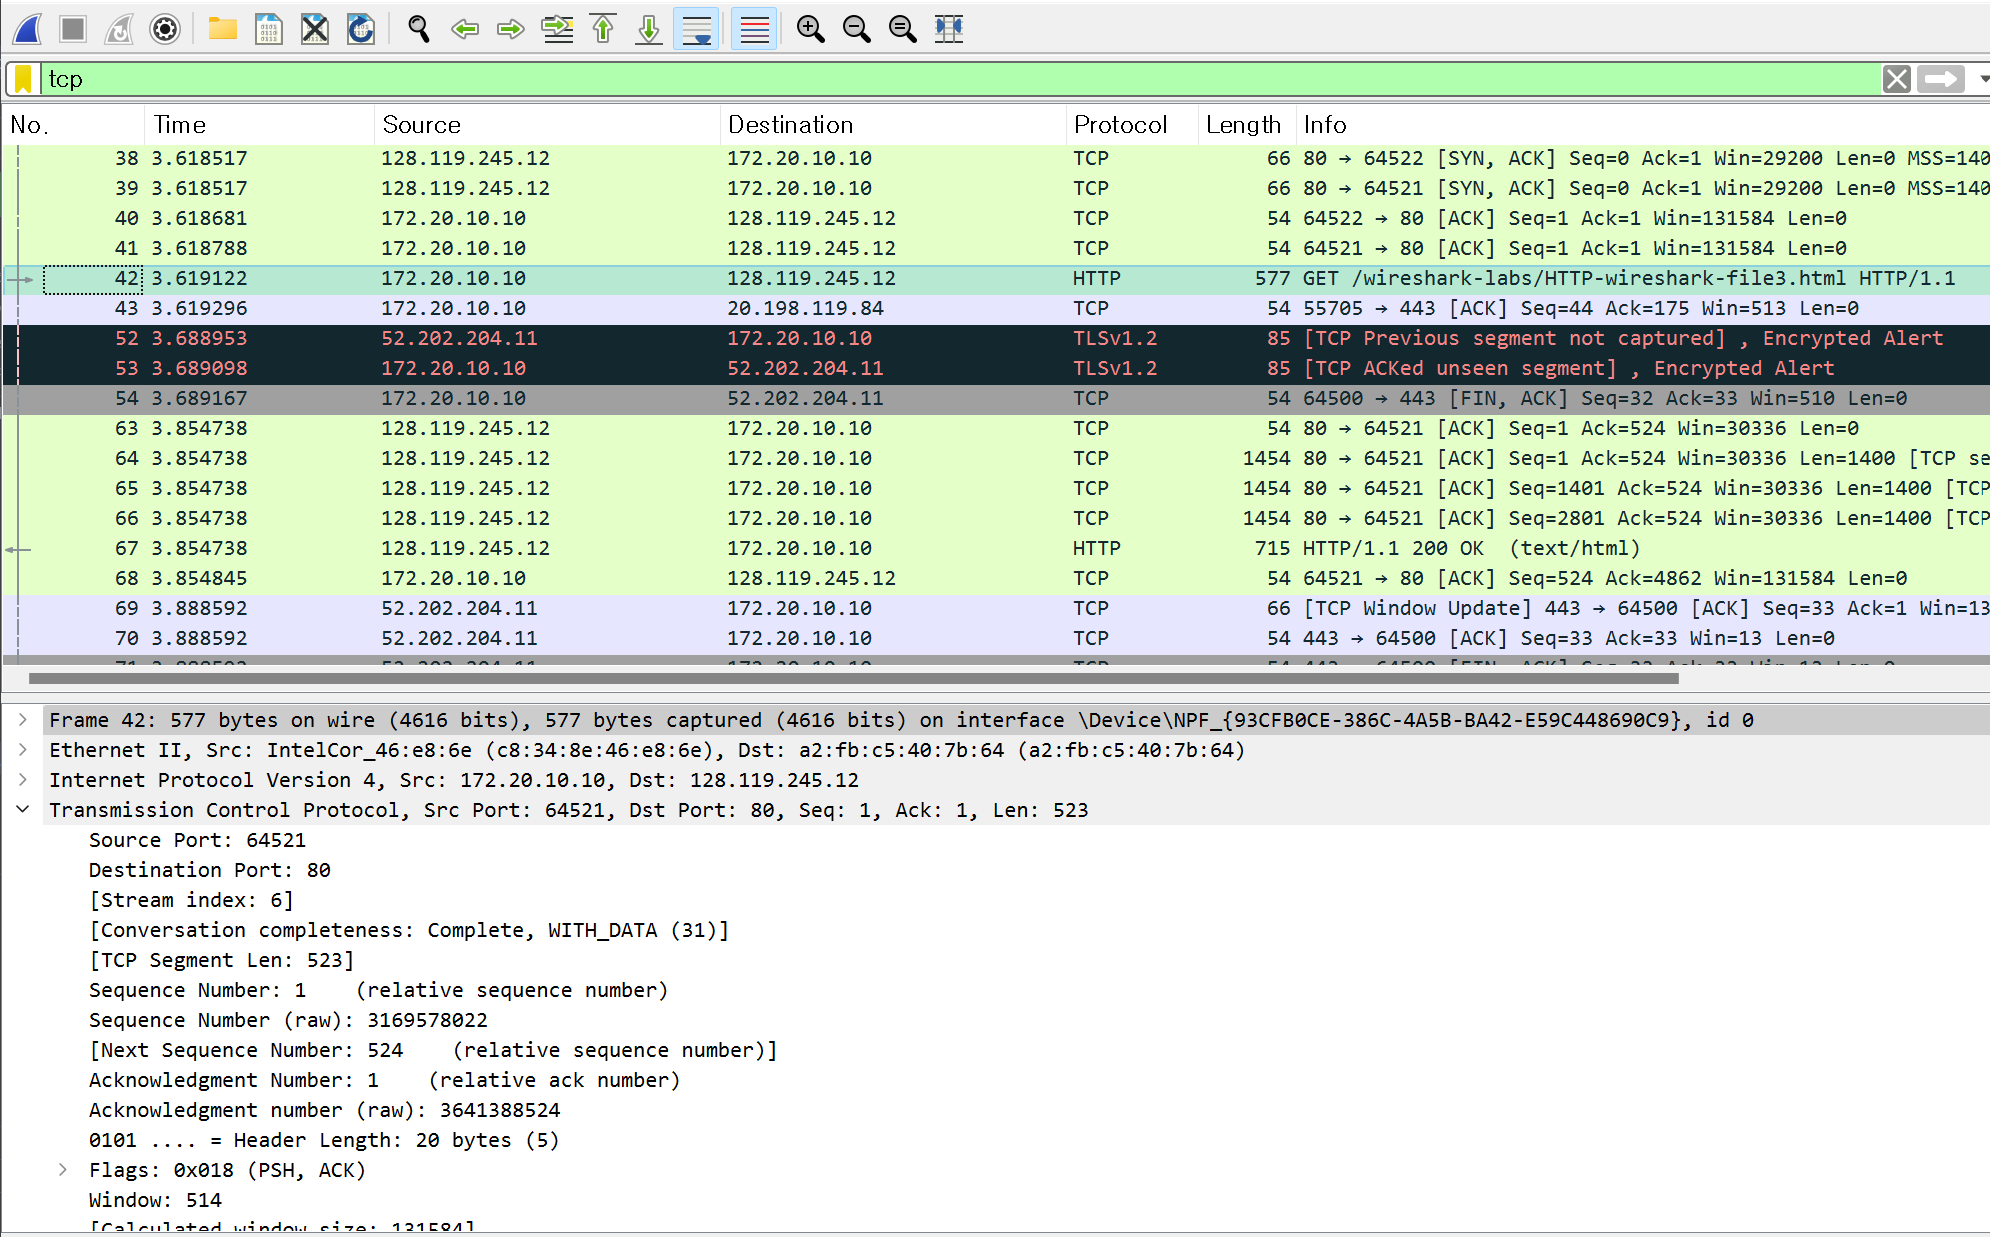
\includegraphics[width=.95\textwidth]{image/week01/2-9.png}
    		\caption{Wireshark Screenshot}
    	\end{figure}
        \vspace{-4mm}  
    \subsubsection*{Questions}
        \begin{enumerate}[label=\bfseries Problem \arabic*:,leftmargin=*,labelindent=1em]
        \addtocounter{enumi}{7}
            \item What is the destination port for the DNS query message? 
            What is the source port of DNS response message?\\[0.2mm]
            \soln
            
            \item To what IP address is the DNS query message sent? 
            Is this the IP address of your default local DNS server?\\[0.2mm]
            \soln
            
            \item Examine the DNS query message. What “Type” of DNS query is it? 
            Does the query message contain any “answers”?\\[0.2mm]
            \soln
            
            \item Examine the DNS response message. 
            How many “answers” are provided? What do each of these answers contain?\\[0.2mm]
            \soln
            
        \end{enumerate}
% Experiment 3-3
\subsection{DNS : Traing DNS with Wireshark \#3}
    \subsubsection*{Experiment Results}
         \vspace{-4mm}
    	\begin{figure}[!h]\centering
    % 		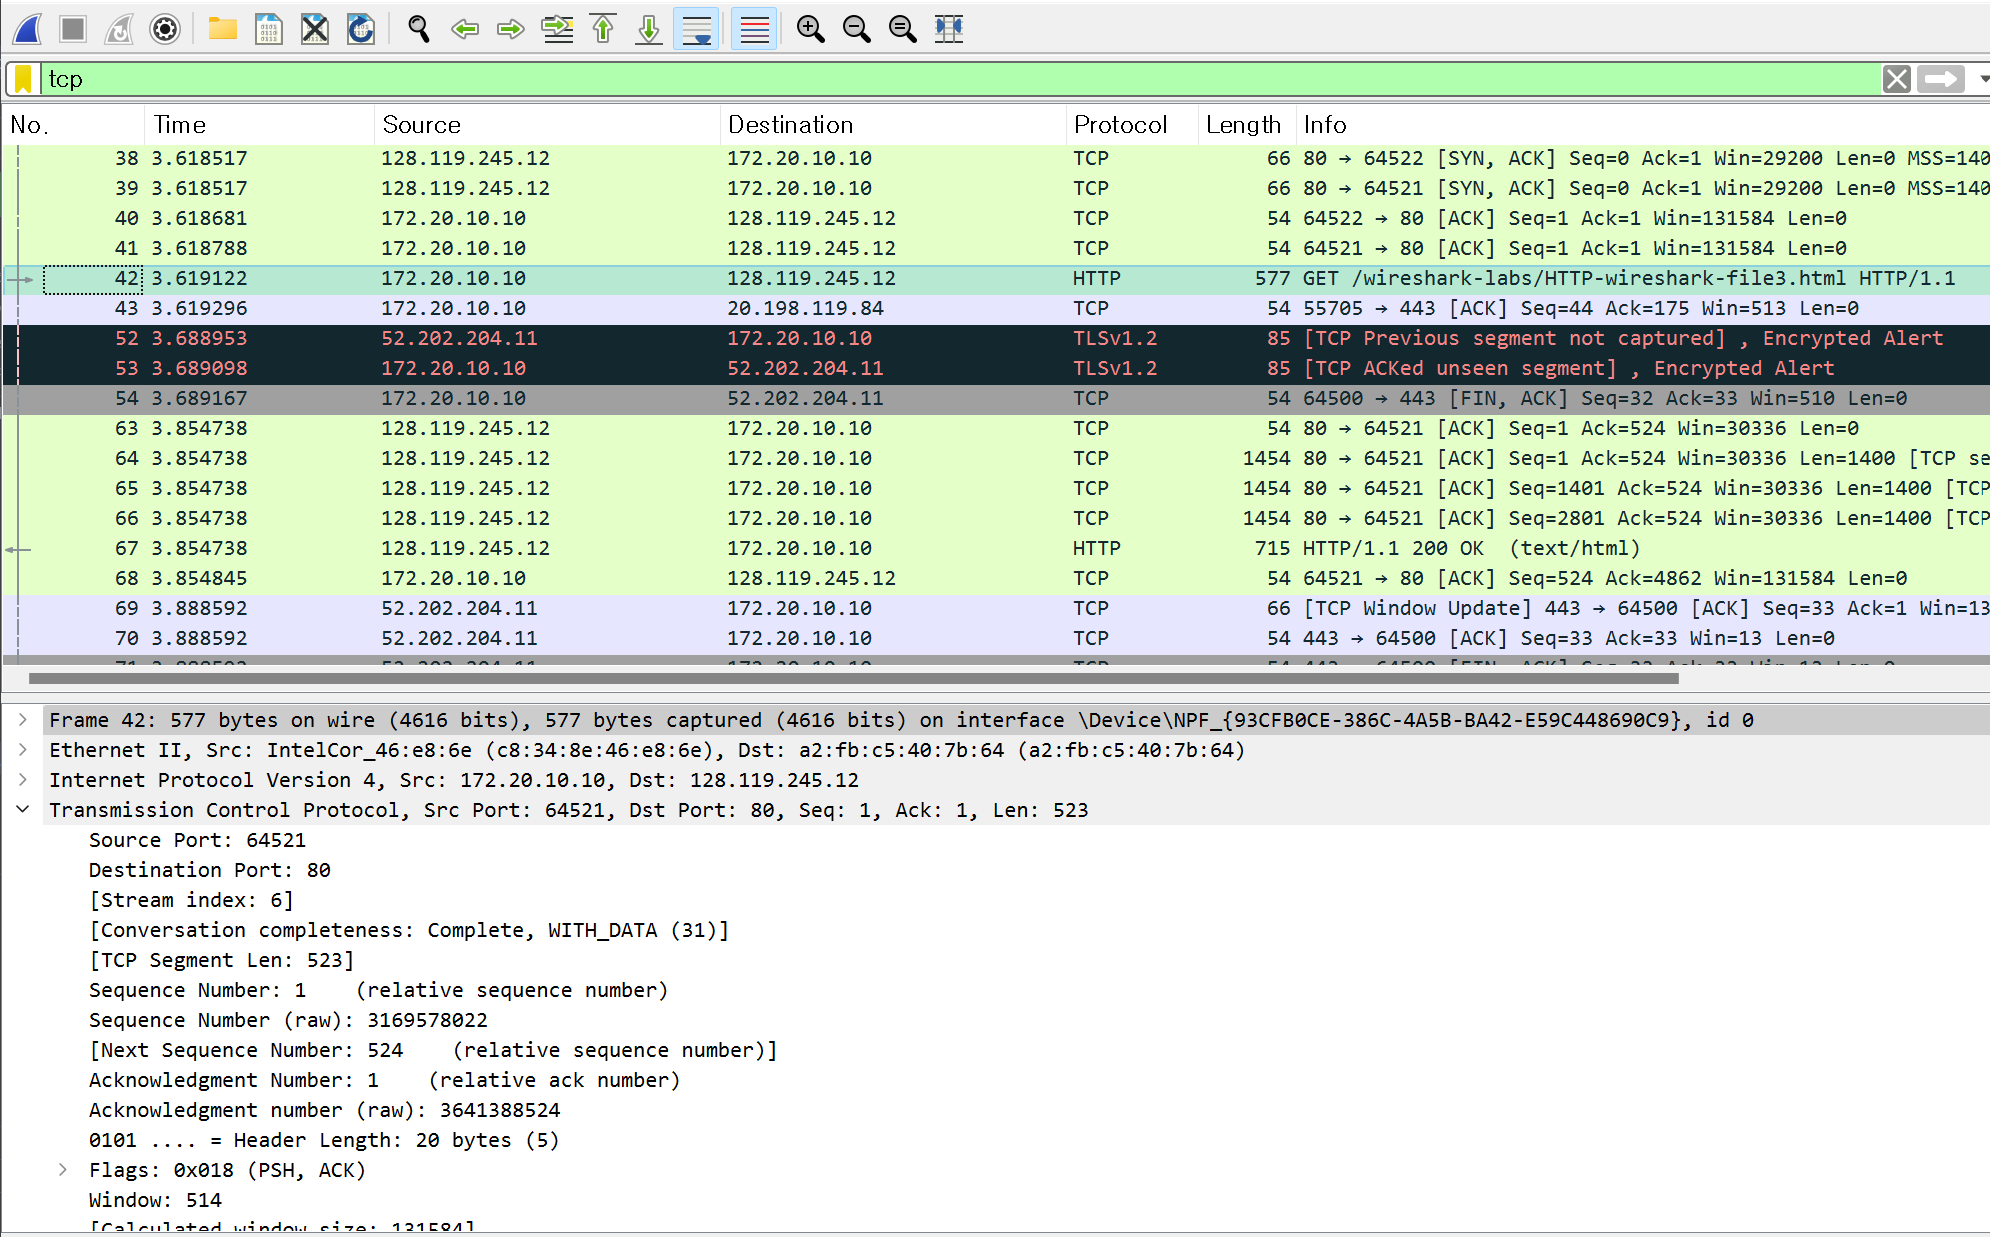
\includegraphics[width=.95\textwidth]{image/week01/2-9.png}
    		\caption{Wireshark Screenshot}
    	\end{figure}
        \vspace{-4mm}  
    \subsubsection*{Questions}
        \begin{enumerate}[label=\bfseries Problem \arabic*:,leftmargin=*,labelindent=1em]
        \addtocounter{enumi}{11}
            \item To what IP address is the DNS query message sent? 
            Is this the IP address of your default local DNS server?\\[0.2mm]
            \soln
            
            \item Examine the DNS query message. What “Type” of DNS query is it? 
            Does the query message contain any “answers”?\\[0.2mm]
            \soln
            
            \item Examine the DNS response message. What MIT nameservers does the response message provide? 
            Does this response message also provide the IP addresses of the MIT nameservers?\\[0.2mm]
            \soln
            
        \end{enumerate}
% Experiment 3-4
\subsection{DNS : Traing DNS with Wireshark \#4}
    \subsubsection*{Experiment Results}
    	\begin{figure}[!h]\centering
    % 		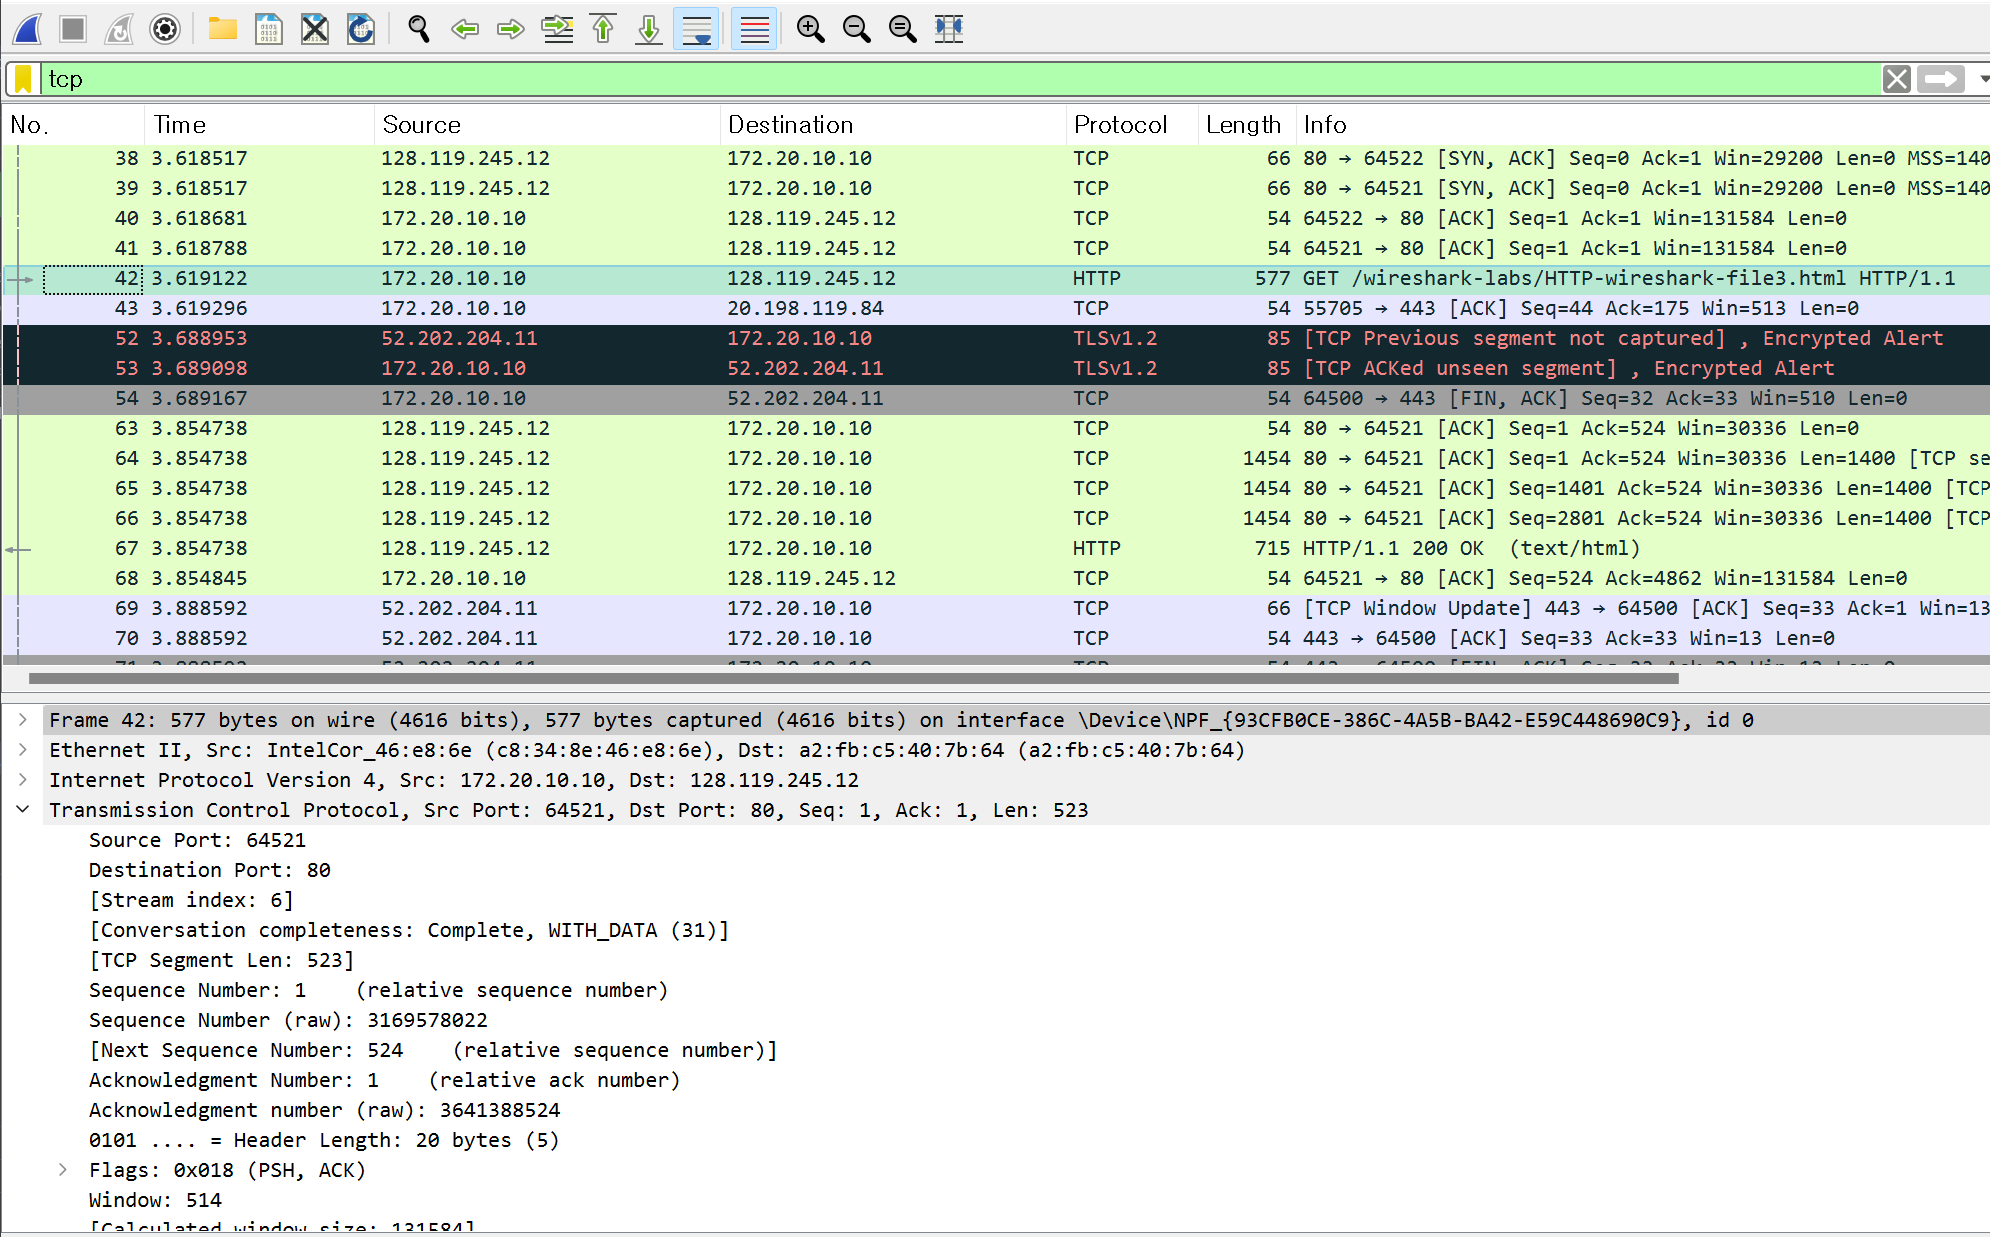
\includegraphics[width=.95\textwidth]{image/week01/2-9.png}
    		\caption{Wireshark Screenshot}
    	\end{figure}
        \vspace{-4mm}  
    \subsubsection*{Questions}
        \begin{enumerate}[label=\bfseries Problem \arabic*:,leftmargin=*,labelindent=1em]
        \addtocounter{enumi}{14}
            \item To what IP address is the DNS query message sent? 
            Is this the IP address of your default local DNS server? 
            If not, what does the IP address correspond to?\\[0.2mm]
            \soln
            
            \item Examine the DNS query message. 
            What “Type” of DNS query is it? Does the query message contain any “answers”?\\[0.2mm]
            \soln
            
            \item Examine the DNS response message. How many “answers” are provided?
            What does each of these answers contain?\\[0.2mm]
            \soln
        \end{enumerate}